\chapter*{Preface}

This piece of notes covers one way of building a \textbf{static} website. It facilitates my live teaching sessions or my Web \& Git YouTube series.
\vspace{6mm}

We use \textbf{Pug.js} (sometimes abbreviated to Pug in this piece of notes) instead of HTML, \textbf{less} instead of CSS. And used gulp to translate the files back to HTML and CSS. The generated HTML files can be directly opened by the browser. We also included \textbf{Bootstrap} to make our static website responsive.
\vspace{6mm}

At the same time, we will be learning how to use \textbf{Git} and \textbf{command line tools}.

\section{Prerequisites}

Basic coding experience (e.g. variables, loops) in any programming languages (e.g. C++, Python) is expected. Knowing basic HTML and CSS would be helpful, but not a must. I would contrast HTML with Pug.js and CSS with less throughout the notes, if you have not learned HTML and CSS you could skip those sessions.

\section{Way to read the notes}

This piece of notes aims to fill the gaps of the online resources, and also acts as the bridge between different components of the project. It will not include every detail that you need to know, but I would try to include different online resources (documentations and YouTube tutorials) required in the form of hyperlinks along the way.

\vspace{6mm}

I marked the less essential sections with \textit{Advanced} or \textit{Of less importance}. The whole of \cref{sec:git2} and \cref{sec:pug2} are labelled with \textit{Advanced}, while the whole of \cref{sec:misc} is labelled with \textit{Of less importance}. You can read the sections without the markings first, then those with \textit{Advanced}, then those with \textit{Of less importance}.

\section{Why?}

I would like to explain what I would like to achieve this piece of notes in this section, so as to manage your expectations.
\vspace{6mm}

\textbf{TL;DR: I believe what you will learn is useful in some way if you would like to pursue jobs related to IT, or dig deeper in programming and Computer Science. Knowledge in Git is also crucial for Maths, Statistics and science subjects undergraduates as they also need to write code sometimes as a group.}

\subsection*{Why making websites?}

Websites are cross-platform, meaning that they can be opened on different kinds of devices, basically any device with a browser. From mobile phones to laptops and desktops, no matter which operating system they are on (e.g. Windows, MacOS, Linux, Android, iOS).

On the other hand, you can only code mobile apps for one specific platform\footnote{Flutter or React Native are exceptions, but they have their downsides}. For instance, Android apps I built cannot be installed on iOS devices unfortunately.

\subsection*{Command line and Git}

Learning how to make a website is actually just a facade. The most important thing that I think you will take away with is the knowledge on command line and Git.

Knowing how to use the command line is important because you can work more efficiently if you are proficient at command line tools. And you will come across some situations where only command line is available (e.g. when accessing a remote server). 

Git is important because it allows you to work and communicate with people using just a few simple commands. By following its rules and conventions, you can work with others efficiently, without having to send zip files back and forth through emails. 

\subsection*{Can I use GitHub Desktop or similar visualisation tools in place for command line?}

Not really. Git is a command line tool and is best used through the command line. Again, you will come across some situations where only command line is available (e.g. when accessing a remote server). 

However, it is acceptable if you just want to visualise the git commit history. Just don't run any commands using those visualisation software. (See \cref{sec:sublime})

\subsection*{Why not plain HTML?}

Pug.js allows the use of templates, hence there is no need to modify every page file whenever we need to something that every page has in common. Pug.js also allows the use of variables, so that we can control what to be rendered based on the situation, hence providing a basis for building dynamic websites. (see \cref{sec:limitations} Scope and limitations)

Moreover, using my template allows you to learn about the conventions of Node.js frameworks, such as how \texttt{npm install} works, and the use of files such as \texttt{package.json}. Knowing these makes it slightly easier for you to learn state-of-the-art Node.js frameworks (e.g. React, Angular, Discord.js).

\subsection*{Responsiveness}

Mobile devices are common nowadays, so our website has to cater for screens with different sizes, from those as small as mobile phones to those as big as projectors. 

A website is responsive if it can rearrange its elements for easy readability based on the screen size and orientation. The use of Bootstrap makes our website responsive.
\vspace{6mm}

I think the following summarises what we talked about in this section. I think building websites is half of the course while another half is about command line and Git.

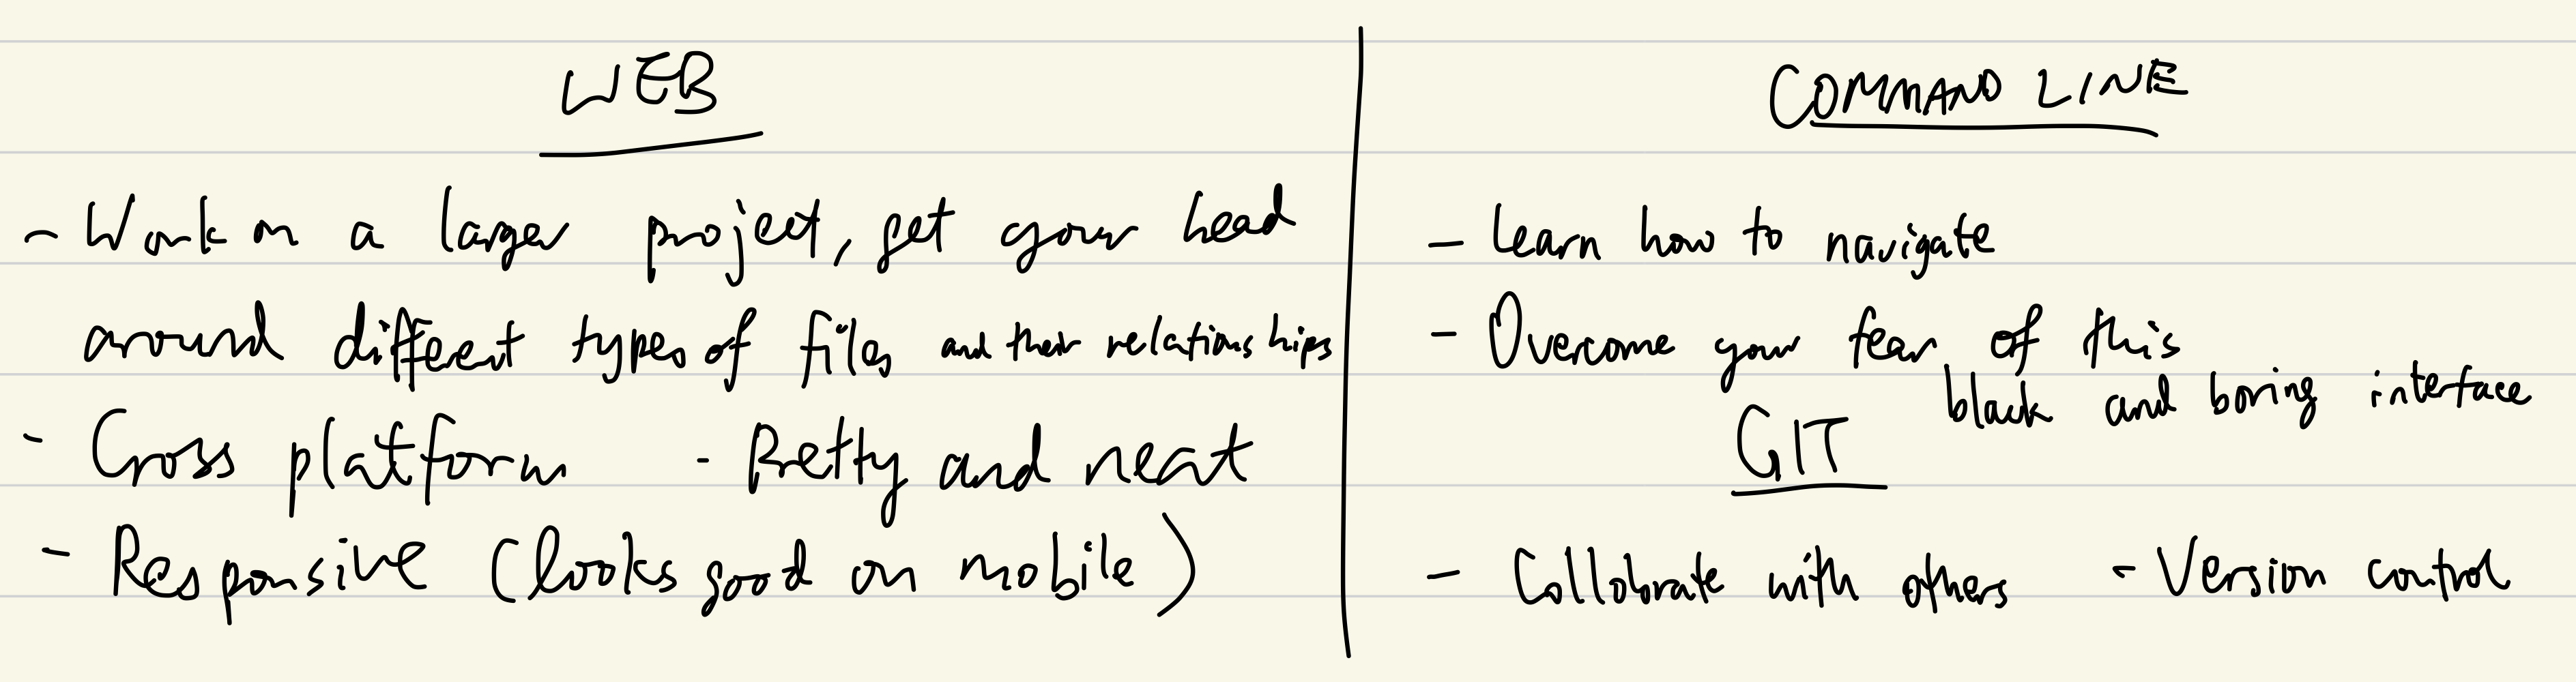
\includegraphics[width=15cm]{images/ch0-summary-of-course.png}

\section{Scope and limitations}
\label{sec:limitations}
We will focus on styling and making the web page responsive. Our styles would be neat, but without too many animations, making them suitable for serious applications such as e-commerce, or a self-introduction website, while not too suitable for websites for fun.

We will not focus much on providing interactions with users, so JavaScript is not used throughout this piece of notes, however, you could definitely add interactions on your own.

The websites that we are making are static. That means we cannot interact with back-end servers and databases securely, while dynamic websites can. A framework that you can learn after mastering this piece of notes is \href{https://expressjs.com/}{ExpressJS}.\footnote{Link: \url{https://expressjs.com/}}

\section{A word of warning}

This is just a draft, aiming to include everything in the shortest amount of time possible, so explanations and examples may be inadequate. If there are any errors in the notes feel free to contact me by email oscar.mui@univ.ox.ac.uk

\section{Linktree}

Useful links related to the notes.
\vspace{6mm}

Video series I made: \textit{(I have to admit they are not of the best quality, and the series is not finished yet)}

\url{https://www.youtube.com/playlist?list=PLjGmdnqrOKuYXiu7lgG5HW71jPEUd1XCm}
\vspace{6mm}

Example website:

\url{https://numbersarefun.netlify.app/}
\vspace{6mm}

Template for you to start from scratch:

\url{https://github.com/KidProf/static-web-sandbox}
\vspace{6mm}

Source code of the finished website:

\url{https://github.com/KidProf/numbersarefun-sample-temp}
\vspace{6mm}

Pug.js: 

\url{https://pugjs.org/}
\vspace{6mm}

Less: 

\url{https://lesscss.org/}
\vspace{6mm}

Bootstrap: 

\url{https://getbootstrap.com/}
\vspace{6mm}

